\documentclass[11pt,a4paper]{article}

\usepackage[a4paper,left=2.2cm,right=2.2cm,top=2.4cm,bottom=2.4cm]{geometry}
\usepackage[T1]{fontenc}
\usepackage[utf8]{inputenc}
\usepackage{lmodern}
\usepackage{microtype}
\usepackage{booktabs}
\usepackage{tabularx}
\usepackage{array}
\usepackage{enumitem}
\usepackage{hyperref}
\usepackage{xcolor}
\usepackage{titlesec}
\usepackage{fancyhdr}
\usepackage{lastpage}
\usepackage{tcolorbox}
\usepackage{amsmath}
\usepackage{amssymb}
\usepackage{tikz}
\usetikzlibrary{positioning}
\tcbuselibrary{skins,breakable}

\hypersetup{
  colorlinks=true,
  linkcolor=black,
  urlcolor=black,
  pdftitle={PHOENIX evaluatiestudie - HCP-PRE-04 (C07 + C08)},
  pdfauthor={Stijn Van Severen -- Universiteit Gent}
}

\definecolor{PrimaryBlue}{HTML}{1D4ED8}
\definecolor{DarkBlue}{HTML}{1E3A5F}
\definecolor{SlateMid}{HTML}{475569}
\definecolor{ForestGreen}{HTML}{047857}
\definecolor{RichPurple}{HTML}{6D28D9}
\definecolor{GoldAmber}{HTML}{B45309}
\definecolor{StrongRed}{HTML}{B91C1C}
\definecolor{SoftBG}{HTML}{F8FAFC}
\definecolor{BorderGrey}{HTML}{CBD5E1}
\definecolor{AccentBlue}{HTML}{DBEAFE}
\definecolor{AccentGreen}{HTML}{D1FAE5}
\definecolor{AccentAmber}{HTML}{FEF3C7}
\definecolor{AccentPurple}{HTML}{EDE9FE}
\definecolor{AccentTeal}{HTML}{CCFBF1}

\titleformat{\section}{\Large\bfseries\color{DarkBlue}}{\thesection}{0.7em}{}[\vspace{-0.2em}\color{PrimaryBlue}\rule{\textwidth}{0.6pt}]
\titleformat{\subsection}{\large\bfseries\color{PrimaryBlue}}{\thesubsection}{0.6em}{}
\titleformat{\subsubsection}{\normalsize\bfseries\color{ForestGreen}}{\thesubsubsection}{0.5em}{}

\setlist[itemize]{topsep=3pt,itemsep=2pt,leftmargin=1.4em}
\setlist[enumerate]{topsep=3pt,itemsep=2pt,leftmargin=1.6em}
\setlength{\parskip}{0.45em}
\setlength{\parindent}{0pt}
\renewcommand{\arraystretch}{1.28}

\pagestyle{fancy}
\fancyhf{}
\fancyhead[L]{\small\color{SlateMid}PHOENIX evaluatiestudie -- Fase 1}
\fancyhead[R]{\small\color{SlateMid}\textbf{HCP-PRE-04}\quad C07 + C08}
\fancyfoot[C]{\small Pagina \thepage\ van \pageref{LastPage}}
\renewcommand{\headrulewidth}{0.3pt}
\renewcommand{\footrulewidth}{0pt}

\newtcolorbox{complaintbox}[1][]{
  colback=blue!3,colframe=PrimaryBlue,
  boxrule=0.8pt,arc=2.5mm,breakable,
  left=10pt,right=10pt,top=8pt,bottom=8pt,
  fonttitle=\small\bfseries\color{PrimaryBlue},
  title=Casusvignet,#1
}
\newtcolorbox{contextbox}[1][]{
  colback=green!3,colframe=ForestGreen,
  boxrule=0.6pt,arc=2mm,breakable,
  left=8pt,right=8pt,top=7pt,bottom=7pt,
  fonttitle=\small\bfseries\color{ForestGreen},
  title=Gestandaardiseerde context,#1
}
\newtcolorbox{instrbox}[1][]{
  colback=SoftBG,colframe=BorderGrey,
  boxrule=0.5pt,arc=1.5mm,breakable,
  left=8pt,right=8pt,top=7pt,bottom=7pt,
  fonttitle=\bfseries\color{SlateMid},#1
}
\newtcolorbox{monitorbox}{
  colback=SoftBG,colframe=BorderGrey,
  boxrule=0.5pt,arc=1.5mm,breakable,
  left=6pt,right=6pt,top=5pt,bottom=5pt
}
\newtcolorbox{responsebox}{
  colback=yellow!5,colframe=GoldAmber,
  boxrule=0.7pt,arc=2mm,breakable,
  left=10pt,right=10pt,top=9pt,bottom=9pt,
  fonttitle=\small\bfseries\color{GoldAmber},
  title=Uw antwoord
}

\tikzset{
  crnode/.style={
    draw=PrimaryBlue,fill=AccentBlue,rounded corners=2pt,
    text width=3.55cm,minimum height=0.76cm,
    font=\fontsize{6.5}{8}\selectfont\bfseries\color{DarkBlue},
    align=center,inner sep=3pt
  },
  prnode/.style={
    draw=ForestGreen,fill=AccentTeal,rounded corners=2pt,
    text width=3.55cm,minimum height=0.76cm,
    font=\fontsize{6.5}{8}\selectfont\bfseries\color{ForestGreen},
    align=center,inner sep=3pt
  },
}

\newcommand{\writeline}{\vspace{0.22em}\noindent\rule{\linewidth}{0.25pt}\vspace{0.42em}\par}

\newcommand{\criterionslot}[1]{%
\vspace{0.25em}\noindent
\begin{tcolorbox}[colback=SoftBG,colframe=BorderGrey,boxrule=0.4pt,arc=1.5mm,left=8pt,right=8pt,top=5pt,bottom=5pt]%
\small\textbf{\color{SlateMid}Criterium #1}\hspace{1em}%
\textbf{Label (2--5 woorden):}\hspace{0.5em}\rule{0.50\linewidth}{0.25pt}%
\end{tcolorbox}%
}

\newcommand{\predictorslot}[1]{%
\vspace{0.25em}\noindent
\begin{tcolorbox}[colback=SoftBG,colframe=BorderGrey,boxrule=0.4pt,arc=1.5mm,left=8pt,right=8pt,top=5pt,bottom=5pt]%
\small\textbf{\color{SlateMid}Predictor #1}\hspace{1em}%
\textbf{Label (2--6 woorden):}\hspace{0.5em}\rule{0.50\linewidth}{0.25pt}%
\end{tcolorbox}%
}

\newcommand{\rankbox}[1]{%
\vspace{0.22em}\noindent
\begin{tikzpicture}[baseline=3pt]
  \node[draw=DarkBlue,fill=AccentBlue,rounded corners=3pt,minimum width=2.5cm,minimum height=0.72cm,font=\small\bfseries\color{DarkBlue},align=center] {Prioriteit #1};
\end{tikzpicture}
\hspace{0.7em}\rule{0.60\linewidth}{0.25pt}\par\vspace{0.05em}
}

\newcommand{\checkitemBFS}[2]{%
\noindent\small\textbf{#1.}\hspace{0.45em}$\square$\hspace{0.4em}#2\par\vspace{0.20em}}

\newcommand{\messagelines}{\writeline\writeline\writeline\writeline}

\begin{document}

% ── TITELPAGINA ─────────────────────────────────────────────────────────────
\thispagestyle{fancy}
\vspace*{0.3cm}

\begin{tcolorbox}[
  colback=DarkBlue,colframe=DarkBlue,
  arc=3mm,left=14pt,right=14pt,top=12pt,bottom=12pt,
  width=\textwidth
]
\centering
{\fontsize{22}{28}\selectfont\bfseries\color{white}
PHOENIX evaluatiestudie\\[0.3em]
\fontsize{15}{20}\selectfont\color{AccentBlue}
Fase 1 -- onafhankelijke expertgeneratie\\[0.2em]
\fontsize{12}{16}\selectfont\color{white}
\textit{Instrument voor Zorgprofessionals}
}
\end{tcolorbox}

\vspace{0.6cm}

\begin{center}
\begin{tcolorbox}[
  colback=AccentBlue,colframe=PrimaryBlue,
  arc=2.5mm,boxrule=1.2pt,left=12pt,right=12pt,top=10pt,bottom=10pt,
  width=0.86\textwidth
]
\centering
{\large\bfseries\color{DarkBlue}Deelnemerscode: \texttt{HCP-PRE-04}}\\[0.5em]
{\normalsize\color{SlateMid}
Toegewezen casussen:\quad
\textbf{\color{PrimaryBlue}C07} (46-jarige accountmanager)
\quad en \quad
\textbf{\color{PrimaryBlue}C08} (38-jarige projectmanager)
}
\end{tcolorbox}
\end{center}

\vspace{0.5cm}

\begin{center}
\begin{tcolorbox}[
  colback=SoftBG,colframe=BorderGrey,
  arc=2mm,left=10pt,right=10pt,top=9pt,bottom=9pt,
  width=0.92\textwidth
]
\small\renewcommand{\arraystretch}{1.28}
\begin{tabularx}{\textwidth}{@{}>{\bfseries\raggedright\arraybackslash}p{0.29\textwidth}X@{}}
Studie & Evaluatie van de klinische kwaliteit van een ontologiegebaseerd multi-agentsysteem voor gepersonaliseerde digitale geestelijke gezondheidszorg (PHOENIX) \\
Instelling & Universiteit Gent -- Faculteit Psychologie en Pedagogische Wetenschappen \\
Onderzoeker & Stijn Van Severen (masterproefstudent) \\
Promotoren & Prof.\ Dr.\ Geert Crombez; Dr.\ Annick De Paepe \\
Contact & \texttt{stijn.vanseveren@ugent.be} \\
Geschatte duur & Ongeveer 35--45 minuten voor beide casussen samen \\
\end{tabularx}
\end{tcolorbox}
\end{center}

\vspace{0.4cm}

\begin{center}
\begin{tcolorbox}[
  colback=SoftBG,colframe=BorderGrey,
  arc=2mm,left=10pt,right=10pt,top=9pt,bottom=9pt,
  width=0.92\textwidth
]
\textbf{\color{PrimaryBlue}Doel van deze bundel}

\medskip\small
U neemt deel aan een evaluatiestudie waarin zorgprofessionals onafhankelijk dezelfde
vijf klinische redeneerstappen uitvoeren als het PHOENIX-systeem. Uw antwoorden
vormen het menselijke referentiecorpus voor een latere dubbelblinde vergelijking
met systeemoutput.

\smallskip
Voor elk van uw twee casussen vult u dezelfde vijf delen in: (1) operationalisering,
(2) initieel observatiemodel, (3) prioritering van behandeldoelen, (4) verfijning van
EMA-metingen en (5) een mobiele coachingsboodschap.

\smallskip
\textbf{We vragen uw eigen klinische oordeelsvorming.} Antwoord zoals u dat in een
reele professionele context zou doen, maar werk strikt volgens de instructies op de
volgende pagina.
\end{tcolorbox}
\end{center}

\vspace{0.4cm}

\begin{center}
\begin{tcolorbox}[
  colback=AccentAmber,colframe=GoldAmber,
  arc=2mm,boxrule=0.7pt,left=10pt,right=10pt,top=8pt,bottom=8pt,
  width=0.90\textwidth
]
\small\centering
\textbf{\color{GoldAmber}Vertrouwelijkheid:} uw antwoorden worden voor analyse
geanonimiseerd en uitsluitend gebruikt binnen deze masterproefstudie. Deelname is
vrijwillig; u kan zich op elk moment terugtrekken door contact op te nemen met de
onderzoeker.
\end{tcolorbox}
\end{center}

\vfill
\newpage
\tableofcontents
\newpage


% ── INSTRUCTIEPAGINA ─────────────────────────────────────────────────────────
\section{Instructiepagina}

\subsection*{Het PHOENIX-systeem en de context van deze studie}

\textbf{PHOENIX} (Personalized Hierarchical Optimization Engine for Navigating
Insightful eXplorations) is een multi-agentsysteem ontwikkeld als onderdeel van
een masterproef in de psychologie aan de Universiteit Gent. Het systeem verwerkt
een vrije klachttekst en doorloopt vijf opeenvolgende klinische redeneerstappen
die de kern vormen van een gepersonaliseerde, longitudinale digitale interventie.

Het theoretische kader van PHOENIX steunt op het \textbf{netwerk-analytisch model
van psychopathologie} (Borsboom \& Cramer, 2013): psychische klachten worden niet
als uitingen van een latente stoornis beschouwd, maar als een \emph{dynamisch
netwerk van onderling samenhangende klachtcomponenten}. Een sleutelbegrip daarbinnen
is het onderscheid tussen \textbf{criteria} (symptoomdimensies die de toestand van
de persoon beschrijven) en \textbf{predictoren} (modificeerbare variabelen die de
criteria causaal beinvloeden en als behandeldoel kunnen dienen).

\vspace{0.4em}
\begin{instrbox}[title={Kerndefinities: criterium versus predictor}]
\small
\textbf{Criterium (CR):} een klinisch relevante, momentaan aanwezige
\emph{klacht- of toestandsdimensie} van de persoon die herhaald meetbaar is via
dagelijkse EMA. Criteria zijn de \emph{uitkomstvariabelen} in het netwerk -- ze
beschrijven \emph{wat er mis gaat} (bijv.\ inslaapproblemen, paniekepisoden,
sombere stemming). Criteria zijn geen gedragingen of interventies.

\medskip
\textbf{Predictor (P):} een \emph{modificeerbare gedrags- of procesvariabele}
die plausibel causaal ingrijpt op een of meerdere criteria en dagelijks meetbaar
is via een korte EMA-vraag. Predictoren zijn de \emph{ingreepvariabelen} in het
netwerk -- ze beschrijven \emph{wat veranderbaar is} (bijv.\ avondschermtijd,
geplande exposure, aerobe beweging). Een predictor is \emph{nooit een symptoom zelf},
maar een gedrag, strategie of omgevingsfactor die het symptoom beinvloedt.

\medskip\small
\textit{Voorbeelden ter verduidelijking:}
\begin{itemize}[topsep=1pt,itemsep=0pt]
\item \textbf{Criterium:} inslaapproblemen, anticipatieangst, anergie, guilt-driven ruminatie.
\item \textbf{Predictor:} avondschermtijd (min), geplande exposurestap (ja/nee),
bewegingsfrequentie (min), preslaap-offloading (ja/nee).
\item \textbf{Geen predictor, geen criterium:} eetlust bij avondmaal, rusthartslag,
spierspanning -- dit zijn symptoom- of toestandsmaten, geen behandelbare predictoren.
\end{itemize}
\end{instrbox}

\vspace{0.4em}
\begin{instrbox}[title={Ecological Momentary Assessment (EMA) -- basisprincipes}]
\small
\textbf{EMA} is een methode waarbij personen meerdere keren per dag hun actuele
toestand of gedrag rapporteren via een mobiele applicatie. In PHOENIX wordt EMA
gebruikt om zowel criteria als predictoren dagelijks te monitoren over een periode
van meerdere weken.

Een goede EMA-variabele voldoet aan vier vereisten:
\begin{itemize}[topsep=2pt,itemsep=1pt]
\item \textbf{Dagelijks rapporteerbaar:} via een korte vraag op de smartphone (ja/nee, aantal, minuten of 0--10).
\item \textbf{Dynamisch en veranderbaar:} geen vaste trek, diagnose of stabiel achtergrondkenmerk.
\item \textbf{Klinisch relevant:} toont binnen-persoonsvariatie die therapeutisch informatief is.
\item \textbf{Onderscheid criterium vs.\ predictor:} symptoomdimensies zijn criteria; modificeerbare gedragingen zijn predictoren.
\end{itemize}
\end{instrbox}

\vspace{0.4em}
\begin{instrbox}[title={Het bipartiet netwerk: structuur van het observatiemodel}]
\small
Na 21 dagen EMA-monitoring construeert PHOENIX een \textbf{bipartiet netwerk}:
een graaf met twee kolommensets en gewogen verbindingen daartussen.
\begin{itemize}[topsep=2pt,itemsep=1pt]
\item \textbf{Linkse kolom -- Predictoren (P):} de modificeerbare variabelen.
\item \textbf{Rechtse kolom -- Criteria (CR):} de klacht- en toestandsdimensies.
\item \textbf{Kanten:} de richting loopt van predictor naar criterium (P $\rightarrow$ CR).
Een \emph{blauwe} rand duidt op een positief verband (predictor vergroot het criterium),
een \emph{rode} rand op een negatief verband (predictor verkleint het criterium).
Lijndikte is proportioneel aan de sterkte van het empirische verband uit de monitoringdata.
\end{itemize}
In \textbf{Deel 3} rangschikt u de predictoren op behandelprioriteit op basis van
dit netwerk en de monitoringsamenvatting.
\end{instrbox}

\vspace{0.5em}

\subsection*{Overzicht van de vijf taken}

\begin{center}
\renewcommand{\arraystretch}{1.36}
\small
\begin{tabular}{@{}>{\bfseries\color{PrimaryBlue}}p{0.05\textwidth}>{\bfseries}p{0.30\textwidth}p{0.38\textwidth}p{0.13\textwidth}@{}}
\toprule
Stap & Klinische taak & Wat u doet & Richttijd \\
\midrule
1 & Operationalisering & Identificeer 2--6 \textbf{criteriumlabels} (klachtdimensies) & $\approx$\,6 min \\
2 & Initieel observatiemodel & Genereer 3--5 \textbf{predictorlabels} (modificeerbaar, EMA-geschikt) & $\approx$\,6 min \\
3 & Behandeldoelprioritering & Rangschik alle 5 \textbf{predictoren} van hoog naar laag behandelprioriteit & $\approx$\,7 min \\
4 & Verfijnd observatiemodel & Selecteer exact 6 \textbf{EMA-items} (2 per behandeldoel) uit de lijst van 20 & $\approx$\,8 min \\
5 & Mobiele coaching & Schrijf een korte patient\-gerichte boodschap voor de app & $\approx$\,8 min \\
\midrule
 & \textbf{Totaal (2 casussen)} & & \textbf{35--45 min} \\
\bottomrule
\end{tabular}
\end{center}

\vspace{0.5em}
\begin{instrbox}[title={Werkwijze -- strikt te volgen}]
\begin{enumerate}[topsep=1pt,itemsep=2pt]
\item \textbf{Werk sequentieel: Deel 1 $\rightarrow$ Deel 5.}
Ga pas naar een volgend deel wanneer het huidige deel volledig is afgewerkt voor beide casussen.
\item \textbf{Gebruik geen generatieve AI, schrijfhulpmiddelen, richtlijnen of collegaoverleg.}
Extern gebruik ondermijnt de methodologische validiteit en de blind scoringswaarde van de studie.
\item \textbf{Gebruik in latere delen uitsluitend de meegeleverde gestandaardiseerde context.}
Die is bewust vastgezet zodat alle deelnemers op identieke input reageren en vergelijkbaar zijn.
\item \textbf{Herwerk eerdere antwoorden niet retroactief} nadat u latere context hebt gezien.
\item \textbf{Noteer of typ rechtstreeks in de voorziene antwoordzones.}
Onleesbare of ambigu geformuleerde antwoorden bemoeilijken latere blinde beoordeling.
\end{enumerate}
\end{instrbox}

\newpage


\section{Deel 1: Operationalisering van de mentale gezondheidstoestand}

\begin{tcolorbox}[colback=blue!3,colframe=PrimaryBlue,arc=2.5mm,boxrule=0.9pt,
  left=10pt,right=10pt,top=9pt,bottom=9pt]
\textbf{\color{PrimaryBlue}Instructies Deel 1}

\smallskip\small
\textbf{Opdracht:} identificeer de belangrijkste actuele klacht- en toestandsdimensies
(\textbf{criteria}) in de klachttekst en noteer voor elke dimensie uitsluitend een
\textbf{kort criteriumlabel}.

\textbf{Wat is een criterium?}
Een criterium is een \emph{symptoom- of klachtdimensie} die beschrijft \emph{wat er
mis gaat} bij de persoon. Het is \emph{geen} behandeling, geen gedrag en geen oorzaak,
maar een actuele toestandsbeschrijving:
\begin{itemize}[topsep=2pt,itemsep=1pt]
\item momenteel aanwezig bij de persoon (niet hypothetisch of anamnestisch),
\item onderscheidbaar van andere klachtdimensies (niet overlappend),
\item in principe herhaald meetbaar via dagelijkse zelfrapportage (EMA).
\end{itemize}

\textbf{Voorbeelden van goede criteriumlabels:}
inslaapproblemen, paniekepisoden, anticipatieangst, sombere stemming, emotionele uitputting,
anergie, interpersoonlijke instabiliteit, compulsief controleergedrag.

\textbf{Let op:} gedragingen (bijv. ``avondschermtijd''), oorzaken (bijv. ``werkstress'')
en behandelstrategieën zijn \emph{geen} criteria maar predictoren -- die horen in Deel 2.

\textbf{Antwoordformat:} label van 2--5 woorden, zonder beschrijvende zin.
Noteer per casus \textbf{2--6 criteria}. Laat ongebruikte velden leeg.
\end{tcolorbox}

\vspace{0.5em}

\newpage

\subsection*{Casus 1: 46-jarige accountmanager}

\begin{complaintbox}[title={Casus 1: 46-jarige accountmanager; duur: 14 maanden}]
\small ``Al meer dan een jaar word ik de meeste ochtenden wakker met een zwaar en vlak gevoel. Het is niet eens intense verdrietigheid, eerder een aanhoudende grijsheid waardoor niets nog de moeite lijkt. Heel eenvoudige taken voelen enorm zwaar aan: mij aankleden, een mail beantwoorden, een maaltijd maken. Ik ben stilaan het contact verloren met bijna iedereen met wie ik vroeger omging, omdat ik de energie niet heb om relaties te onderhouden. Ik slaap veel maar voel mij nooit uitgerust. In stilte vraag ik mij af of ik ooit nog de oude zal worden. Mijn huisarts heeft mij aangeraden hulp te zoeken.''
\end{complaintbox}

\begin{responsebox}
\small\textbf{Opdracht:} noteer \textbf{2--6 criteriumlabels} voor deze casus.
Gebruik enkel korte labels; voeg geen beschrijving toe.

\criterionslot{1}
\criterionslot{2}
\criterionslot{3}
\criterionslot{4}
\criterionslot{5}
\criterionslot{6}
\end{responsebox}

\vspace{0.6em}

\newpage

\subsection*{Casus 2: 38-jarige projectmanager}

\begin{complaintbox}[title={Casus 2: 38-jarige projectmanager; duur: sinds de kindertijd, duidelijk verergerd in de voorbije 12 maanden}]
\small ``Ik heb altijd al moeite gehad om mij te concentreren op taken die mij niet meteen interesseren, maar het is het voorbije jaar veel erger geworden. Ik begin aan projecten en maak ze zelden af. Ik vergeet afspraken, zelfs als ik ze ergens noteer. Mijn partner is gefrustreerd omdat ik volgens hem of haar niet echt luister en onbetrouwbaar overkom. Ik weet dat ik op veel vlakken competent ben, maar ik voel mij voortdurend een mislukking. Ik ben taken die moeilijk zullen zijn ook steeds meer beginnen vermijden, waardoor de achterstand alleen maar groter wordt.''
\end{complaintbox}

\begin{responsebox}
\small\textbf{Opdracht:} noteer \textbf{2--6 criteriumlabels} voor deze casus.
Gebruik enkel korte labels; voeg geen beschrijving toe.

\criterionslot{1}
\criterionslot{2}
\criterionslot{3}
\criterionslot{4}
\criterionslot{5}
\criterionslot{6}
\end{responsebox}

\vspace{0.6em}

\newpage


\section{Deel 2: Initieel observatiemodel (bipartiet netwerk)}

\begin{tcolorbox}[colback=green!3,colframe=ForestGreen,arc=2.5mm,boxrule=0.9pt,
  left=10pt,right=10pt,top=9pt,bottom=9pt]
\textbf{\color{ForestGreen}Instructies Deel 2}

\smallskip\small
\textbf{Opdracht:} genereer \textbf{3--5 predictorlabels} die samen het
\textbf{initieel observatiemodel} voor deze casus vormen.

\textbf{Wat is een predictor in deze context?}
Een predictor is een \emph{modificeerbare gedrags- of procesvariabele} die beschrijft
\emph{wat de persoon kan veranderen}:
\begin{itemize}[topsep=2pt,itemsep=1pt]
\item \textbf{Modificeerbaar:} de persoon (of therapeut) kan er rechtstreeks op ingrijpen.
\item \textbf{EMA-geschikt:} dagelijks meetbaar via een eenvoudige vraag op de smartphone
(ja/nee, aantal, minuten of 0--10 schaal).
\item \textbf{Causaal plausibel:} klinisch aannemelijk dat het predictor de criteria beinvloedt.
\item \textbf{Geen criterium:} symptomen, klachtniveaus of diagnostische trekken zijn
\emph{geen} predictoren.
\end{itemize}

\textbf{Voorbeelden van goede predictorlabels:}
avondschermtijd, geplande exposure, aerobe beweging, preslaap-offloading,
veiligheidsgedrag, werk-privegrens, herstelactiviteit, compulsie-uitstel.

\textbf{Let op:} predictoren als ``eetlust'', ``spierspanning'' of ``moeheid'' zijn
symptoomdimensies (criteria) -- geen predictoren. Kies variabelen die de persoon
actief kan uitvoeren of aanpassen.

\textbf{Antwoordformat:} enkel een label van 2--6 woorden, zonder meetdefinitie of toelichting.
Laat ongebruikte velden leeg.
\end{tcolorbox}

\vspace{0.5em}

\newpage
\subsection*{Casus 1: 46-jarige accountmanager -- Deel 2}

\begin{complaintbox}[title={Casus 1: verkorte klachtomschrijving}]
\small 46-jarige accountmanager; duur: 14 maanden. Aanhoudende sombere stemming, anergie, sociale isolatie en hopeloosheid over herstel.
\end{complaintbox}

\begin{contextbox}
\small\textbf{Gestandaardiseerde criteria uit stap 1:}
\begin{itemize}[topsep=2pt,itemsep=1pt]
\item \textbf{CR-1} Aanhoudende sombere stemming
\item \textbf{CR-2} Anergie
\item \textbf{CR-3} Sociale isolatie
\item \textbf{CR-4} Hopeloosheid
\end{itemize}
\end{contextbox}

\begin{responsebox}
\small\textbf{Opdracht:} noteer \textbf{3--5 predictorlabels} voor een initieel observatiemodel.
Zorg dat elk label later dagelijks via een mobiele app meetbaar kan worden gemaakt.

\predictorslot{1}
\predictorslot{2}
\predictorslot{3}
\predictorslot{4}
\predictorslot{5}
\end{responsebox}

\vspace{0.6em}
\newpage
\subsection*{Casus 2: 38-jarige projectmanager -- Deel 2}

\begin{complaintbox}[title={Casus 2: verkorte klachtomschrijving}]
\small 38-jarige projectmanager; duur: sinds de kindertijd, duidelijk verergerd in de voorbije 12 maanden. Aandachtsvolhoudingsproblemen, plannings- en organisatiefouten, interpersoonlijke onoplettendheid en prestatieschaamte.
\end{complaintbox}

\begin{contextbox}
\small\textbf{Gestandaardiseerde criteria uit stap 1:}
\begin{itemize}[topsep=2pt,itemsep=1pt]
\item \textbf{CR-1} Aandachtsvolhoudingsproblemen
\item \textbf{CR-2} Plannings- en organisatiefouten
\item \textbf{CR-3} Interpersoonlijke onoplettendheid
\item \textbf{CR-4} Prestatieschaamte
\end{itemize}
\end{contextbox}

\begin{responsebox}
\small\textbf{Opdracht:} noteer \textbf{3--5 predictorlabels} voor een initieel observatiemodel.
Zorg dat elk label later dagelijks via een mobiele app meetbaar kan worden gemaakt.

\predictorslot{1}
\predictorslot{2}
\predictorslot{3}
\predictorslot{4}
\predictorslot{5}
\end{responsebox}

\vspace{0.6em}
\newpage


\section{Deel 3: Behandeldoelprioritering via het bipartiet netwerk}

\begin{tcolorbox}[colback=yellow!5,colframe=GoldAmber,arc=2.5mm,boxrule=0.9pt,
  left=10pt,right=10pt,top=9pt,bottom=9pt]
\textbf{\color{GoldAmber}Instructies Deel 3}

\smallskip\small
\textbf{Opdracht:} rangschik de \textbf{5 standaardpredictoren} van \textbf{hoogste}
naar \textbf{laagste} behandelprioriteit.

\textbf{Wat is een behandeldoel?}
Een behandeldoel is de predictor die, als hij veranderd wordt, naar verwachting de sterkste
vermindering van de criteria oplevert. U selecteert op basis van drie criteria:
\begin{enumerate}[topsep=2pt,itemsep=1pt,label=\alph*)]
\item \textbf{Bewijs uit monitoring:} is er in de monitoringdata aanleiding dat deze predictor
actief bijdraagt aan de klacht (bijv.\ hoge frequentie van problematisch gedrag, of bijna
afwezigheid van gewenst gedrag)?
\item \textbf{Klinische modificeerbaarheid:} is de predictor realistisch veranderbaar voor
deze persoon, gegeven profiel en context?
\item \textbf{Netwerkimpact:} beïnvloedt de predictor meerdere criteria tegelijk (hogere
return-on-intervention)?
\end{enumerate}

\textbf{Het bipartiet netwerk lezen:}
\begin{itemize}[topsep=2pt,itemsep=1pt]
\item Predictoren staan in de \textbf{linkerkolom (groen)}; criteria in de \textbf{rechterkolom (blauw)}.
\item \textbf{Blauwe rand:} predictor heeft een positief verband met het criterium
(hogere predictor $\rightarrow$ hoger criterium; bijv.\ meer veiligheidsgedrag $\rightarrow$ meer angst).
\item \textbf{Rode rand:} predictor heeft een negatief verband met het criterium
(hogere predictor $\rightarrow$ lager criterium; bijv.\ meer exposure $\rightarrow$ minder vermijding).
\item \textbf{Lijndikte:} proportioneel aan de sterkte van het empirische verband
(21-daagse EMA-data).
\end{itemize}

\textbf{Antwoordformat:} vul alle 5 prioriteitslijnen in, van rangorde 1 (hoogste prioriteit)
tot en met 5 (laagste prioriteit).
\end{tcolorbox}

\vspace{0.5em}

\newpage
\subsection*{Casus 1: 46-jarige accountmanager -- Deel 3}

\begin{complaintbox}[title={Casus 1: 46-jarige accountmanager}]
\small Aanhoudende sombere stemming, anergie, sociale isolatie en hopeloosheid over herstel. Duur: 14 maanden.
\end{complaintbox}

\begin{monitorbox}
\small\textbf{21-daagse monitoring:} Voltooiingsgraad van geplande activiteiten: 28\%. Sociale contactmomenten/week: gem. 0,8. Stemming: gem. 2,9/10. Variatie in slaap-waaktijd: gem. 2,3 uur. Plezierige activiteiten: gem. 0,9/dag. Uitdagen van hopeloze gedachten: gem. 0,6/dag.
\end{monitorbox}

\begin{center}
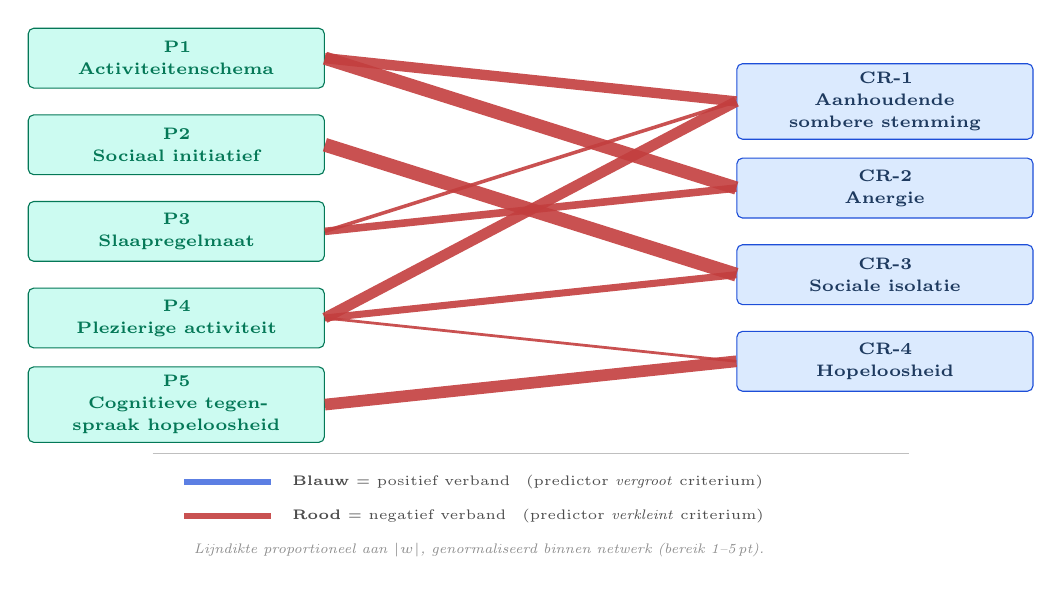
\begin{tikzpicture}[node distance=0pt]
  \node[prnode] (p1) at (0, 2.2) {P1\\Activiteitenschema};
  \node[prnode] (p2) at (0, 1.1) {P2\\Sociaal initiatief};
  \node[prnode] (p3) at (0, 0.0) {P3\\Slaapregelmaat};
  \node[prnode] (p4) at (0, -1.1) {P4\\Plezierige activiteit};
  \node[prnode] (p5) at (0, -2.2) {P5\\Cognitieve tegenspraak hopeloosheid};
  \node[crnode] (cr1) at (9, 1.65) {CR-1\\Aanhoudende sombere stemming};
  \node[crnode] (cr2) at (9, 0.55) {CR-2\\Anergie};
  \node[crnode] (cr3) at (9, -0.55) {CR-3\\Sociale isolatie};
  \node[crnode] (cr4) at (9, -1.65) {CR-4\\Hopeloosheid};
  \draw[line width=5.0pt, draw=StrongRed!85, opacity=0.90] (p2.east) -- (cr3.west);
  \draw[line width=4.79pt, draw=StrongRed!85, opacity=0.90] (p1.east) -- (cr2.west);
  \draw[line width=4.23pt, draw=StrongRed!85, opacity=0.90] (p5.east) -- (cr4.west);
  \draw[line width=3.88pt, draw=StrongRed!85, opacity=0.90] (p4.east) -- (cr1.west);
  \draw[line width=2.54pt, draw=StrongRed!85, opacity=0.90] (p4.east) -- (cr3.west);
  \draw[line width=3.74pt, draw=StrongRed!85, opacity=0.90] (p1.east) -- (cr1.west);
  \draw[line width=2.75pt, draw=StrongRed!85, opacity=0.90] (p3.east) -- (cr2.west);
  \draw[line width=1.0pt, draw=StrongRed!85, opacity=0.90] (p4.east) -- (cr4.west);
  \draw[line width=1.28pt, draw=StrongRed!85, opacity=0.90] (p3.east) -- (cr1.west);
  % Legend (3 stacked rows)
  \draw[line width=0.3pt, draw=black!25] (-0.3, -2.82) -- (9.3, -2.82);
  \draw[line width=2.2pt, draw=PrimaryBlue!80, opacity=0.90] (0.1, -3.18) -- (1.2, -3.18);
  \node[font=\fontsize{5.5}{7}\selectfont, anchor=west, text=black!70] at (1.35, -3.18) {\textbf{Blauw} = positief verband \enspace (predictor \emph{vergroot} criterium)};
  \draw[line width=2.2pt, draw=StrongRed!85, opacity=0.90] (0.1, -3.62) -- (1.2, -3.62);
  \node[font=\fontsize{5.5}{7}\selectfont, anchor=west, text=black!70] at (1.35, -3.62) {\textbf{Rood} = negatief verband \enspace (predictor \emph{verkleint} criterium)};
  \node[font=\fontsize{5.0}{6.5}\selectfont, anchor=west, text=black!45] at (0.1, -4.05) {\textit{Lijndikte proportioneel aan $|w|$, genormaliseerd binnen netwerk (bereik 1--5\,pt).}};
\end{tikzpicture}
\end{center}

\begin{responsebox}
\small\textbf{Opdracht:} rangschik \textbf{alle 5 predictors} van hoogste naar laagste behandelprioriteit.
\textbf{Beschikbare predictors:} \textbf{P1: Activiteitenschema},\quad \textbf{P2: Sociaal initiatief},\quad \textbf{P3: Slaapregelmaat},\quad \textbf{P4: Plezierige activiteit},\quad \textbf{P5: Cognitieve tegenspraak hopeloosheid}

\rankbox{1}
\rankbox{2}
\rankbox{3}
\rankbox{4}
\rankbox{5}
\end{responsebox}

\vspace{0.6em}
\newpage
\subsection*{Casus 2: 38-jarige projectmanager -- Deel 3}

\begin{complaintbox}[title={Casus 2: 38-jarige projectmanager}]
\small Aandachtsvolhoudingsproblemen, plannings- en organisatiefouten, interpersoonlijke onoplettendheid en prestatieschaamte. Duur: sinds de kindertijd, duidelijk verergerd in de voorbije 12 maanden.
\end{complaintbox}

\begin{monitorbox}
\small\textbf{21-daagse monitoring:} Gestarte versus afgewerkte taken: 68\% versus 29\%. Gemiste afspraken of toezeggingen: gem. 2,1/week. Partnerconflicten: gem. 4,7/week. Externe tools gebruikt: gem. 1,8/dag. Positieve zelfbekrachtiging: gem. 0,4/dag.
\end{monitorbox}

\begin{center}
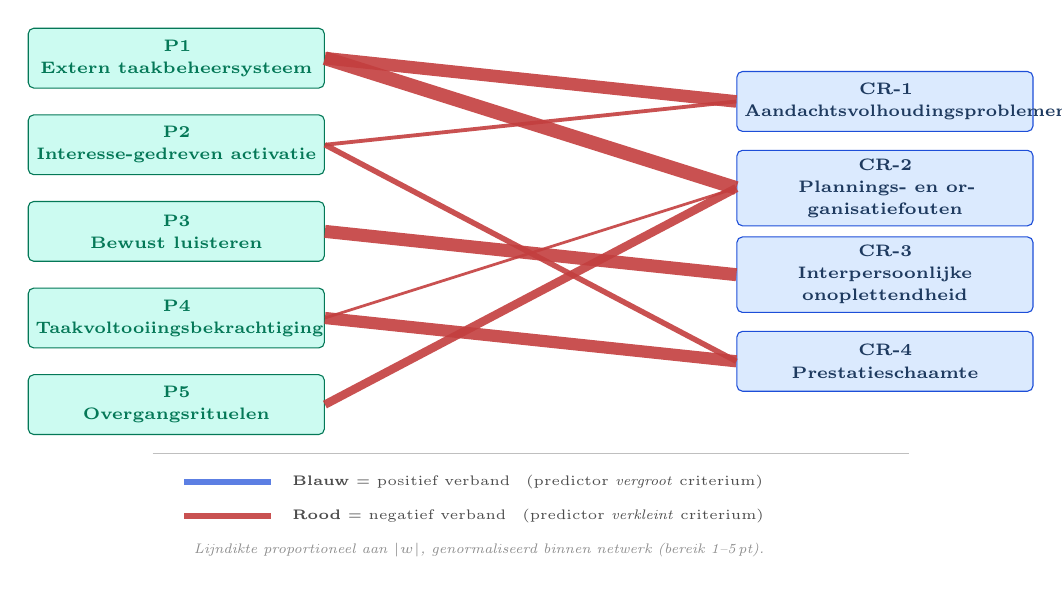
\begin{tikzpicture}[node distance=0pt]
  \node[prnode] (p1) at (0, 2.2) {P1\\Extern taakbeheersysteem};
  \node[prnode] (p2) at (0, 1.1) {P2\\Interesse-gedreven activatie};
  \node[prnode] (p3) at (0, 0.0) {P3\\Bewust luisteren};
  \node[prnode] (p4) at (0, -1.1) {P4\\Taakvoltooiingsbekrachtiging};
  \node[prnode] (p5) at (0, -2.2) {P5\\Overgangsrituelen};
  \node[crnode] (cr1) at (9, 1.65) {CR-1\\Aandachtsvolhoudingsproblemen};
  \node[crnode] (cr2) at (9, 0.55) {CR-2\\Plannings- en organisatiefouten};
  \node[crnode] (cr3) at (9, -0.55) {CR-3\\Interpersoonlijke onoplettendheid};
  \node[crnode] (cr4) at (9, -1.65) {CR-4\\Prestatieschaamte};
  \draw[line width=5.0pt, draw=StrongRed!85, opacity=0.90] (p1.east) -- (cr2.west);
  \draw[line width=4.7pt, draw=StrongRed!85, opacity=0.90] (p3.east) -- (cr3.west);
  \draw[line width=4.55pt, draw=StrongRed!85, opacity=0.90] (p1.east) -- (cr1.west);
  \draw[line width=4.4pt, draw=StrongRed!85, opacity=0.90] (p4.east) -- (cr4.west);
  \draw[line width=3.04pt, draw=StrongRed!85, opacity=0.90] (p5.east) -- (cr2.west);
  \draw[line width=1.98pt, draw=StrongRed!85, opacity=0.90] (p2.east) -- (cr4.west);
  \draw[line width=1.38pt, draw=StrongRed!85, opacity=0.90] (p2.east) -- (cr1.west);
  \draw[line width=1.0pt, draw=StrongRed!85, opacity=0.90] (p4.east) -- (cr2.west);
  % Legend (3 stacked rows)
  \draw[line width=0.3pt, draw=black!25] (-0.3, -2.82) -- (9.3, -2.82);
  \draw[line width=2.2pt, draw=PrimaryBlue!80, opacity=0.90] (0.1, -3.18) -- (1.2, -3.18);
  \node[font=\fontsize{5.5}{7}\selectfont, anchor=west, text=black!70] at (1.35, -3.18) {\textbf{Blauw} = positief verband \enspace (predictor \emph{vergroot} criterium)};
  \draw[line width=2.2pt, draw=StrongRed!85, opacity=0.90] (0.1, -3.62) -- (1.2, -3.62);
  \node[font=\fontsize{5.5}{7}\selectfont, anchor=west, text=black!70] at (1.35, -3.62) {\textbf{Rood} = negatief verband \enspace (predictor \emph{verkleint} criterium)};
  \node[font=\fontsize{5.0}{6.5}\selectfont, anchor=west, text=black!45] at (0.1, -4.05) {\textit{Lijndikte proportioneel aan $|w|$, genormaliseerd binnen netwerk (bereik 1--5\,pt).}};
\end{tikzpicture}
\end{center}

\begin{responsebox}
\small\textbf{Opdracht:} rangschik \textbf{alle 5 predictors} van hoogste naar laagste behandelprioriteit.
\textbf{Beschikbare predictors:} \textbf{P1: Extern taakbeheersysteem},\quad \textbf{P2: Interesse-gedreven activatie},\quad \textbf{P3: Bewust luisteren},\quad \textbf{P4: Taakvoltooiingsbekrachtiging},\quad \textbf{P5: Overgangsrituelen}

\rankbox{1}
\rankbox{2}
\rankbox{3}
\rankbox{4}
\rankbox{5}
\end{responsebox}

\vspace{0.6em}
\newpage


\section{Deel 4: Verfijnd observatiemodel -- selectie van sub-predictoren}

\begin{tcolorbox}[colback=purple!4,colframe=RichPurple,arc=2.5mm,boxrule=0.9pt,
  left=10pt,right=10pt,top=9pt,bottom=9pt]
\textbf{\color{RichPurple}Instructies Deel 4}

\smallskip\small
\textbf{Opdracht:} selecteer per casus \textbf{exact 6 EMA-items}:
\textbf{2 sub-predictoren per behandeldoel} (3 behandeldoelen $\times$ 2 = 6 items).

\textbf{Wat zijn sub-predictoren?}
Een behandeldoel uit Deel 3 (bijv.\ ``geplande exposure'') is een conceptueel label.
In de volgende EMA-cyclus moet dit label vertaald worden naar \emph{concrete, dagelijks
meetbare gedragsitems} -- de \textbf{sub-predictoren}. Elke sub-predictor is een
specifieke operationalisering van het behandeldoel als dagelijkse EMA-vraag.

\textbf{Voorbeeld:} behandeldoel = \textit{avondschermtijd}
$\rightarrow$ sub-predictor 1: ``smartphone-gebruik na 22.00 uur (min)''
$\rightarrow$ sub-predictor 2: ``schermvrij interval voor slapengaan (min)''

\textbf{Belangrijk: alle 20 items in de lijst zijn predictor-type EMA-items}
(modificeerbare gedragingen en strategieën -- \emph{geen} symptomen of
klachtdimensies). Uw taak is te selecteren welke 6 items het best aansluiten bij
de 3 gestandaardiseerde behandeldoelen, 2 per doel.

\textbf{Selectieprincipe:}
\begin{itemize}[topsep=2pt,itemsep=1pt]
\item Kies per behandeldoel de 2 items die dat doel het meest direct en precies meten.
\item Verkies items die samen een compleet beeld geven van het behandeldoel
(bijv.\ frequentie \emph{en} duur, of twee complementaire gedragingen).
\item Vermijd items die het behandeldoel slechts zijdelings raken.
\end{itemize}

\textbf{Antwoordformat:} vink \textbf{exact 6} items aan. Geen toelichting vereist.
\end{tcolorbox}

\vspace{0.5em}

\newpage
\subsection*{Casus 1: 46-jarige accountmanager -- Deel 4}

\begin{contextbox}
\small\textbf{Gestandaardiseerde behandeldoelen uit Deel 3:}
\begin{enumerate}[topsep=2pt,itemsep=1pt,label=\arabic*.]
\item \textbf{Activiteitenschema}\quad\textit{\small (lage voltooiingsgraad (28\%); gedragsactivatie is hier het primaire mechanisme)}
\item \textbf{Slaapregelmaat}\quad\textit{\small (sterke variatie in slaap-waakritme verstoort stemming en energieregulatie)}
\item \textbf{Sociaal initiatief}\quad\textit{\small (gemiddeld 0,8 contacten/week; essentieel voor CR-3 en indirect voor stemming)}
\end{enumerate}
\end{contextbox}

\begin{responsebox}
\small\textbf{Opdracht:} selecteer \textbf{exact 6} EMA-items (2 per behandeldoel) die het best passen als volgende subpredictoren.
\textit{Alle antwoordopties zijn dagelijkse mobiele EMA-items.}

\checkitemBFS{1}{Cafeine-inname na 15.00 uur (aantal)}
\checkitemBFS{2}{Geplande activiteit uit dagschema bewust uitgevoerd (ja/nee)}
\checkitemBFS{3}{Ontbijt op vaste tijd bewust genuttigd (ja/nee)}
\checkitemBFS{4}{Aantal geplande activiteiten daadwerkelijk uitgevoerd vandaag (aantal)}
\checkitemBFS{5}{Werkgerelateerde gedachten bewust gestopt of beperkt in de avond (min)}
\checkitemBFS{6}{Lichte lichaamsbeweging of stretching om energie te verhogen (min)}
\checkitemBFS{7}{Opstaan op geplande wektijd aangehouden (ja/nee)}
\checkitemBFS{8}{Schermtijd op sociale media bewust beperkt (min)}
\checkitemBFS{9}{Afwijking van geplande bedtijd (min)}
\checkitemBFS{10}{Alcoholinname vanavond (eenheden)}
\checkitemBFS{11}{Middagdutje genomen (ja/nee)}
\checkitemBFS{12}{Gestructureerde taaklijst opgesteld en bijgehouden (ja/nee)}
\checkitemBFS{13}{Bewust contact opgenomen met een kennis of vriend (ja/nee)}
\checkitemBFS{14}{Plezierige activiteit bewust gepland en voltooid (ja/nee)}
\checkitemBFS{15}{Hopeloosheidsgedachten bewust uitgedaagd met een alternatief (ja/nee)}
\checkitemBFS{16}{Duur van sociaal contact op eigen initiatief (min)}
\checkitemBFS{17}{Waterinname vandaag (glazen)}
\checkitemBFS{18}{Bewuste stap tegen vermijding van moeilijke taak gezet (ja/nee)}
\checkitemBFS{19}{Maaltijdmoment op vaste tijd aangehouden (ja/nee)}
\checkitemBFS{20}{Ochtendbeweging of buitenlucht vóór aanvang van de dag (min)}
\vspace{0.4em}
\noindent\textbf{Totaal geselecteerd:}\hspace{0.5em}\rule{1.2cm}{0.25pt}\hspace{0.2em}/ 6
\end{responsebox}

\vspace{0.6em}
\newpage
\subsection*{Casus 2: 38-jarige projectmanager -- Deel 4}

\begin{contextbox}
\small\textbf{Gestandaardiseerde behandeldoelen uit Deel 3:}
\begin{enumerate}[topsep=2pt,itemsep=1pt,label=\arabic*.]
\item \textbf{Extern taakbeheersysteem}\quad\textit{\small (inconsistent gebruik (1,8/dag) terwijl dit de kernscaffolding vormt voor CR-1 en CR-2)}
\item \textbf{Bewust luisteren}\quad\textit{\small (partnerconflicten zijn frequent; direct relevant voor CR-3)}
\item \textbf{Taakvoltooiingsbekrachtiging}\quad\textit{\small (bijna afwezig; kan de schaamtecyclus en vermijding doorbreken)}
\end{enumerate}
\end{contextbox}

\begin{responsebox}
\small\textbf{Opdracht:} selecteer \textbf{exact 6} EMA-items (2 per behandeldoel) die het best passen als volgende subpredictoren.
\textit{Alle antwoordopties zijn dagelijkse mobiele EMA-items.}

\checkitemBFS{1}{Cafeine-inname voor de middag (aantal)}
\checkitemBFS{2}{To-dolijst of digitale planner bewust geraadpleegd (ja/nee)}
\checkitemBFS{3}{Consistent slaap- en waktijdstip aangehouden (ja/nee)}
\checkitemBFS{4}{Nieuwe taken direct en volledig ingevoerd in het taakbeheersysteem (ja/nee)}
\checkitemBFS{5}{Schermtijd voor sociale media tijdens werkuren bewust beperkt (min)}
\checkitemBFS{6}{Korte beweeg- of rekpauze tijdens de werkdag bewust genomen (min)}
\checkitemBFS{7}{Actief luisteren bewust geoefend tijdens een gesprek (ja/nee)}
\checkitemBFS{8}{Notificaties bewust uitgeschakeld tijdens focusblokken (ja/nee)}
\checkitemBFS{9}{Afleiding actief weggelegd of uitgeschakeld tijdens een gesprek (ja/nee)}
\checkitemBFS{10}{Constructieve reactie bewust gekozen na ontvangen kritiek of feedback (ja/nee)}
\checkitemBFS{11}{Lunchpauze bewust en schermvrij genomen (ja/nee)}
\checkitemBFS{12}{Afgesloten taak bewust en expliciet positief erkend (ja/nee)}
\checkitemBFS{13}{Alcoholinname vanavond (eenheden)}
\checkitemBFS{14}{Plezierige activiteit of hobby buiten werk bewust uitgevoerd (min)}
\checkitemBFS{15}{Kleine symbolische beloning gegeven na taakvoltooiing (ja/nee)}
\checkitemBFS{16}{Stappentelling overdag (stappen)}
\checkitemBFS{17}{Ochtendlichtblootstelling of buitengaan in de ochtend (min)}
\checkitemBFS{18}{Middagdutje genomen (ja/nee)}
\checkitemBFS{19}{Geplande vrije activiteit actief bijgewoond of uitgevoerd (ja/nee)}
\checkitemBFS{20}{Waterinname vandaag (glazen)}
\vspace{0.4em}
\noindent\textbf{Totaal geselecteerd:}\hspace{0.5em}\rule{1.2cm}{0.25pt}\hspace{0.2em}/ 6
\end{responsebox}

\vspace{0.6em}
\newpage


\section{Deel 5: Gepersonaliseerde mobiele coachingsboodschap (HAPA-kader)}

\begin{tcolorbox}[colback=red!3,colframe=ForestGreen,arc=2.5mm,boxrule=0.9pt,
  left=10pt,right=10pt,top=9pt,bottom=9pt]
\textbf{\color{ForestGreen}Instructies Deel 5}

\smallskip\small
\textbf{Opdracht:} schrijf een korte, rechtstreeks tot de persoon gerichte
coachingsboodschap die in de mobiele applicatie verschijnt.

\textbf{Theoretisch kader -- HAPA:}
PHOENIX gebruikt het \textbf{Health Action Process Approach (HAPA; Schwarzer, 1992)}
om de boodschap af te stemmen op de motivationele fase van de persoon:
\begin{itemize}[topsep=2pt,itemsep=1pt]
\item \textbf{Pre-intentionele fase:} de persoon is nog niet gemotiveerd om te veranderen
$\rightarrow$ focus op risicobewustzijn en uitkomstverwachting.
\item \textbf{Intentionele fase:} de persoon wil veranderen maar heeft nog geen concreet plan
$\rightarrow$ focus op doelstelling en actieplanning.
\item \textbf{Actie-/onderhoudsfase:} de persoon probeert al te veranderen
$\rightarrow$ focus op copingplanning en zelfeffectiviteitsondersteuning.
\end{itemize}
U hoeft de fase niet expliciet te benoemen; gebruik het kader om de toon en inhoud
van uw boodschap te sturen.

\textbf{De boodschap voldoet aan:}
\begin{itemize}[topsep=2pt,itemsep=2pt]
\item \textbf{Lengte:} 2--4 zinnen, compact genoeg voor een mobiel scherm.
\item \textbf{Toon:} warm, direct, professioneel -- geen klinisch jargon of diagnostische labels.
\item \textbf{Inhoud:} adresseert het primaire behandeldoel en de voornaamste barriere;
bevat een concrete, eerstvolgende actie.
\item \textbf{Perspectief:} tweede persoon (``jij'' of formeel ``u'').
\end{itemize}

\textbf{Werkvoorbeeld} (niet gerelateerd aan een studiecasus):
\begin{tcolorbox}[colback=SoftBG,colframe=BorderGrey,boxrule=0.4pt,arc=1.5mm,
  left=7pt,right=7pt,top=5pt,bottom=5pt]
\small
\textbf{Context:} verpleegkundige; behandeldoel = korte beweegmomenten inbouwen;
barriere = vermoeidheid na de shift (lage zelfeffectiviteit); fase = intentioneel.\\[0.3em]
\textbf{Voorbeeldboodschap:}\\
\textit{``Na een zware shift voelt rust nemen logisch, maar net dat eerste kleine
beweegmoment kan je avond helpen ontladen. Trek vanavond meteen na thuiskomst je
schoenen aan en wandel 10 minuten buiten -- niet meer dan dat ene blokje. Zo maak
je de stap haalbaar en vergroot je de kans dat je lichaam later echt kan afschakelen.''}
\end{tcolorbox}
\end{tcolorbox}

\vspace{0.5em}

\newpage
\subsection*{Casus 1: 46-jarige accountmanager -- Deel 5}

\begin{contextbox}
\small\renewcommand{\arraystretch}{1.24}
\begin{tabular}[t]{@{}>{\raggedright\bfseries\color{ForestGreen}\arraybackslash}p{0.27\linewidth}>{\raggedright\arraybackslash}p{0.67\linewidth}@{}}
Primair probleem & Langdurige sombere stemming en anergie hebben activiteit en sociale verbinding sterk doen afnemen. \\[0.15em]
Behandeldoel & Dagelijks een klein, gepland gedrag uitvoeren als onderdeel van gedragsactivatie. \\[0.15em]
Voornaamste barriere & Planningsdrempel en betekenisverlies: activiteiten voelen vooraf nutteloos en te zwaar. \\[0.15em]
Copingstrategie & Werk met een vooraf gekozen micro-activiteit en een 'klaar is genoeg'-criterium. \\
\end{tabular}
\end{contextbox}

\begin{responsebox}
\small\textbf{Opdracht:} schrijf hieronder de mobiele coachingsboodschap voor deze casus.
\textit{Formuleer alsof de tekst morgen rechtstreeks op de smartphone van de persoon verschijnt.}

\messagelines
\end{responsebox}

\vspace{0.6em}
\newpage
\subsection*{Casus 2: 38-jarige projectmanager -- Deel 5}

\begin{contextbox}
\small\renewcommand{\arraystretch}{1.24}
\begin{tabular}[t]{@{}>{\raggedright\bfseries\color{ForestGreen}\arraybackslash}p{0.27\linewidth}>{\raggedright\arraybackslash}p{0.67\linewidth}@{}}
Primair probleem & Executieve functieproblemen zorgen voor taakfalen, relationele spanning en aanhoudende schaamte. \\[0.15em]
Behandeldoel & Een extern taakbeheersysteem consequent raadplegen en successen expliciet bekrachtigen. \\[0.15em]
Voornaamste barriere & Gewoonteweerstand en lage volhoudingsverwachting: eerdere systemen werden snel losgelaten. \\[0.15em]
Copingstrategie & Installeer een minimale, dagelijks terugkerende check-in en koppel afgeronde taken aan een expliciete bevestiging. \\
\end{tabular}
\end{contextbox}

\begin{responsebox}
\small\textbf{Opdracht:} schrijf hieronder de mobiele coachingsboodschap voor deze casus.
\textit{Formuleer alsof de tekst morgen rechtstreeks op de smartphone van de persoon verschijnt.}

\messagelines
\end{responsebox}

\vspace{0.6em}
\newpage


\section{Afronding en terugbezorging}

Dank u voor het invullen van alle vijf delen voor uw twee toegewezen casussen
(Casus 1 en Casus 2).

\begin{instrbox}[title=Checklist voor terugbezorging]
\begin{itemize}
\item[$\square$] Ik heb in Deel 1 voor beide casussen criteriumlabels ingevuld.
\item[$\square$] Ik heb in Deel 2 voor beide casussen predictorlabels ingevuld.
\item[$\square$] Ik heb in Deel 3 voor beide casussen alle 5 predictors gerangschikt.
\item[$\square$] Ik heb in Deel 4 voor beide casussen exact 6 EMA-items geselecteerd.
\item[$\square$] Ik heb in Deel 5 voor beide casussen een mobiele coachingsboodschap geschreven.
\item[$\square$] Mijn antwoorden weerspiegelen mijn eigen klinische oordeel zonder gebruik van generatieve AI of andere externe hulp.
\item[$\square$] Ik begrijp dat mijn antwoorden geanonimiseerd worden voor analyse.
\end{itemize}
\end{instrbox}

\medskip
Bezorg het ingevulde document terug via e-mail aan:
\begin{center}
\texttt{stijn.vanseveren@ugent.be}\quad met onderwerp:\quad \texttt{PHOENIX-PRE-HCP-PRE-04}
\end{center}

\vspace{0.5em}
\begin{tcolorbox}[colback=AccentBlue,colframe=PrimaryBlue,arc=2mm,boxrule=0.6pt,left=8pt,right=8pt,top=7pt,bottom=7pt]
\small\centering
Na ontvangst worden uw antwoorden geanonimiseerd en opgenomen in het expertreferentiecorpus
voor de latere blind evaluatie van PHOENIX. Hartelijk dank voor uw bijdrage aan dit onderzoek.
\end{tcolorbox}

\end{document}
